

We simulate an FL system with $10$ clients, where the participating clients have different bitwidth configuration and local data distributions. We deploy two bitwidth configurations: (1) the configuration with gradually increasing bitwidth: $20\% 4$-bit, $30\% 6$--bit, $30\% 8$-bit and $20\% 12$-bit models; and (2) the configuration with a skewed bitwidth: $50\% 6$-bit and $50\% 12$-bit models. The experiments involve CIFAR-10 and CIFAR-100 datasets, both for image classification tasks \cite{krizhevsky2009learning}. The datasets are distributed to clients in a non-iid fashion according to Dirichlet$(0.1)$ distribution \cite{bibikar2022federated}.
Simulations were executed on AMD Vega $20$ GPUs. The learning rates were set as in the following prior work: for the supervised learning schemes using low-bit operations we deploy learning rates as in \cite{zhou2016dorefa}, while for self-supervised learning schemes we follow \cite{wang2022does}.
In all simulations, the deployed neural networks were based on ResNet-18 architecture \cite{he2016deep}.
The results are reported after $100$ communication rounds, with clients running $E = 20$ local epochs between any two rounds in CIFAR-10 simulations and $E = 5$ in CIFAR-100 simulations. In the implementation of Fed-QSSL, we rely on the SimCLR method \cite{chen2020simple} for the self-supervision part of the algorithm.\footnote{The codes are available at \url{https://github.com/YiyueC/Fed-QSSL}.}
% Further implementation details are in Appendix.

\begin{table}[t]
\centering
%\resizebox{.95\columnwidth}{!}{
\begin{tabular}{c|c|c}
    \hline
    Algorithm & Global Acc & Local Acc \\
    \hline
    FedAvg & 17.70 & 64.98  \\
    \hline
    FedProx & 14.51 & 68.46  \\
    \hline
    FedPAQ & 16.68 & 62.96  \\
    \hline
    Fed-SimCLR & 39.09 & 77.30  \\
    \hline
    Fed-SimSiam & 36.73 & 76.87 \\
    \hline
    \textbf{Fed-QSSL} & \textbf{59.31} & \textbf{82.50} \\
    \hline 
    \hline
    Fed-SimCLR (Full) & 40.76 & 80.56 \\
    \hline
    \textbf{Fed-QSSL} (Full) & \textbf{72.26} & \textbf{90.01} \\
    \hline
\end{tabular}
\caption{Experiments on CIFAR-10 with model bitwidth configuration $20\% 4$-bit, $30\% 6$--bit, $30\% 8$-bit and $20\% 12$-bit.}
\label{table-1}
\end{table}

\begin{table}[t]
\centering
%\resizebox{.95\columnwidth}{!}{
\begin{tabular}{c|c|c}
    \hline
    Algorithm & Global Acc & Local Acc \\
    \hline
    FedAvg & 20.77 & 66.64  \\
    \hline
    FedProx & 18.70 & 75.60  \\
    \hline
    FedPAQ & 18.56 & 76.57 \\
    \hline
    Fed-SimCLR & 39.12 & 77.43  \\
    \hline
    Fed-SimSiam & 36.44 & 75.21 \\
    \hline
    \textbf{Fed-QSSL} & \textbf{62.26} & \textbf{83.03} \\
    \hline \hline
    Fed-SimCLR (Full) & 40.76 & 80.56 \\
    \hline
    \textbf{Fed-QSSL} (Full) & \textbf{72.26} & \textbf{90.01} \\
    \hline
\end{tabular}
\caption{Experiments on CIFAR-10 with model bitwidth configuration $50\% 6$-bit and $50\% 12$-bit.}
\label{table-2}
\end{table}

\begin{table}[t]
\centering
%\resizebox{.95\columnwidth}{!}{
\begin{tabular}{c|c|c}
    \hline
    Algorithm & Global Acc & Local Acc \\
    \hline
    Fed-SimCLR & 14.79 & 23.46  \\
    \hline
    Fed-SimSiam & 12.24 & 13.59 \\
    \hline
    \textbf{Fed-QSSL} & \textbf{21.44} & \textbf{30.91} \\
    \hline \hline
    Fed-SimCLR (Full) & 15.18 & 30.26 \\
    \hline
    \textbf{Fed-QSSL} (Full) & \textbf{28.75} & \textbf{43.56} \\
    \hline
\end{tabular}
\caption{Experiments on CIFAR-100 with bitwidth configuration $50\% 6$-bit and $50\% 12$-bit.}
\label{table-3}
\end{table}


\begin{figure}
\centering
    \begin{subfigure}
  \centering
  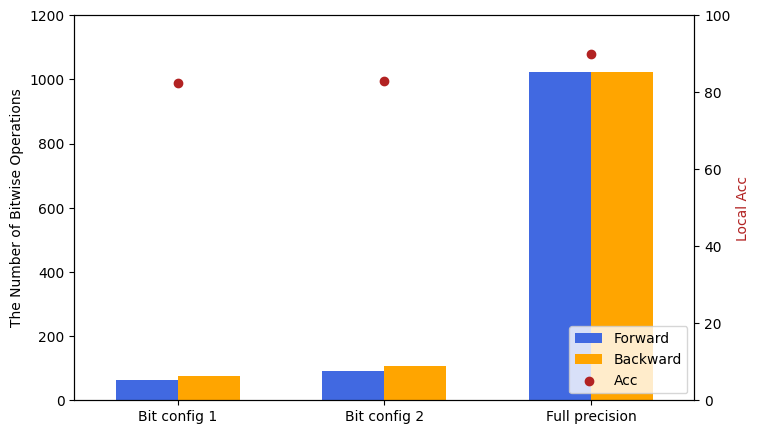
\includegraphics[width=.8\linewidth]{computation_cost.png}
  \caption{The left y-axis indicates the number of bitwise operations while the right y-axis indicates the local accuracy achieved by Fed-QSSL.}
  \label{fig:sfig1}
\end{subfigure}
\vspace{2mm}
\begin{subfigure}
  \centering
  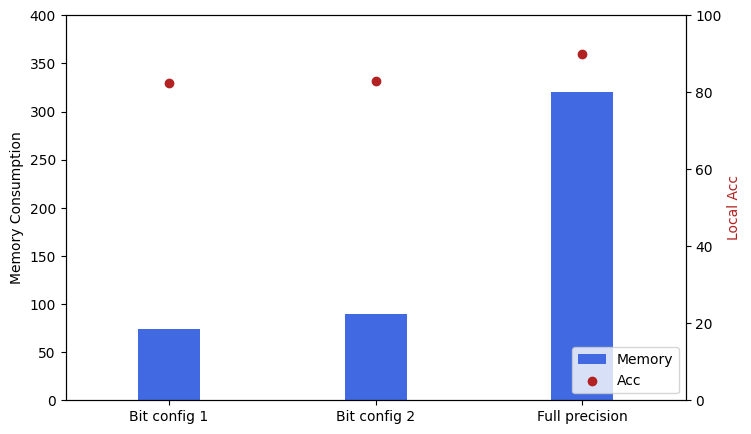
\includegraphics[width=.8\linewidth]{memory_cost_1.png}
  \caption{The left y-axis indicates the memory consumption while the right y-axis indicates the local accuracy achieved by Fed-QSSL.}
  \label{fig:sfig2}
\end{subfigure}
\end{figure}

% \lipsum[1] 
\begin{figure*}
\begin{minipage}[t]{0.3\textwidth}
  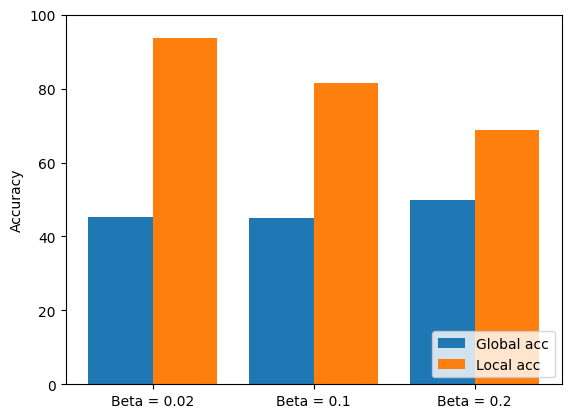
\includegraphics[width=\linewidth]{ab_study_1.png}
  \caption{Ablation study on Dirichlet distribution parameter $\beta$.}
  \label{fig:first}
\end{minipage}%
\hfill % maximize the horizontal separation
\begin{minipage}[t]{0.3\textwidth}
  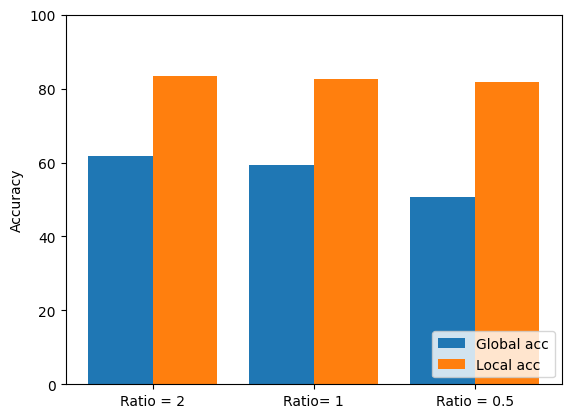
\includegraphics[width=\linewidth]{ab_study_2.png}
  \caption{Ablation study on the ratio of the global buffer size and the local dataset size.}
  \label{fig:second}
\end{minipage}%
\hfill
\begin{minipage}[t]{0.3\textwidth}
  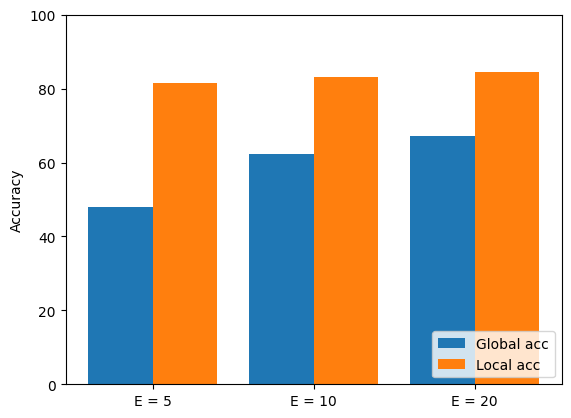
\includegraphics[width=\linewidth]{ab_study_3.png}
  \caption{Ablation study on the number of local training epochs $E$.}
  \label{fig:third}
\end{minipage}%
\end{figure*}

{\bf Baselines.} We compare Fed-QSSL with two groups of algorithms: federated supervised learning (SL) and self-supervised algorithms. The SL algorithms include FedAvg \cite{mcmahan2017communication}, classic FL technique performing simple averaging of local models at each communication round; FedProx \cite{li2020federated}, an FL scheme addressing client data heterogeneity by adding an $\ell_2$-norm regularizer to local objectives to prevent divergence of local updates from the global model; and FedPAQ \cite{reisizadeh2020fedpaq}, a communication-efficient FL algorithm where clients transmit quantized updates to reduce uplink communication cost. As for the SSL algorithms, we consider Fed-SimCLR \cite{chen2020simple,wang2022does} which uses contrastive learning objective to learn a global feature extraction model; and Fed-SimSiam \cite{chen2021exploring} which considers only positive pairs of data points and learn meaningful features by leveraging a feature predictor function and stop-gradient operation. While the baseline algorithms are not originally meant to support local low-bit training, we apply low-bitwidth operations to satisfy resource constraints. In each table of results, the last two rows (labeled as ``Full") correspond to full precision ($32$-bit) models, i.e., models with no bitwidth constraints. 

{\bf Metrics.} Fed-QSSL is compared to the baselines in terms of global accuracy (Global Acc), reflective of robustness, and local accuracy (Local Acc), reflecting personalization. 
%The global accuracy is tested on data coming from uniform distribution. 
SSL methods train a universal linear classifier on top of the frozen global feature extraction model and evaluate the classification accuracy on a uniformly distributed test dataset. Training of a linear classifier to be used for testing global model accuracy is conducted at full precision on a centralized training dataset as in \cite{wang2022does}; this is done only to validate robustness of SSL methods, in real applications no such universal linear classifier is required. SSL methods use the aggregated model and test on uniform testing dataset.
To evaluate local accuracy (i.e., the accuracy on local, generally non-IID datasets), SSL methods train a local linear classifier on top of the frozen low-bitwidth feature extractor while meeting client's bitwidth constraints and run it on a local non-iid testing dataset, while SL methods use a local low-bitwidth classification model and compute the accuracy on local testing data.

{\bf Results.} The results on CIFAR-10 under the first bitwidth configuration are reported in Table \ref{table-1}. Overall, the global accuracy of SSL schemes is higher than SL methods, implying that SSL algorithms tend to learn more accurate representations in data heterogeneous FL scenario. As for the personalization, SSL algorithms achieve higher accuracy on local data, suggesting they learn meaningful representations that are then used in the downstream classification task. It is worth noting that SSL algorithms with higher global accuracy also achieve higher local accuracy; this is because the learned robust feature extractor extracts expressive representations from heterogeneous data which help in downstream classification tasks. Among SL algorithms, however, there exists a trade-off between robustness and personalization, where the performance of models with high global accuracy may suffer locally. Specifically, Fed-QSSL performs better in both bitwidth-heterogeneous and no-constrained (full precision) scenarios due to the use of server-side operations on the global buffer; operations on server facilitate learning robust representations that further improve local performance. Table \ref{table-2} reports results on CIFAR-10 under the second bitwidth configuration. There, SSL algorithms again demonstrate more robust and personalized performance in face of bitwidth and data heterogeneity. As the permitted bitwidth grows, the algorithms reach higher accuracy. Nevertheless, under the bitwidth constraints Fed-QSSL still achieves the highest accuracy. Finally, Table \ref{table-3} reports results on the more challenging CIFAR-100 dataset. As can be seen there, Fed-QSSL perform better than other SSL benchmarks under both low-bitwidth as well as full precision scenarios.

% Might also consider the cost reduction compared to full precision schemes.


{\bf Computation and Memory Saving.}
We next compare the computational cost and memory requirements of Fed-QSSL to those of the full precision scheme. In particular,
for the two bitwidth configurations and the full precision scenario considered above, we report the number of bitwise operations and memory footprint in the local training (see Figure \ref{fig:sfig1} and Figure \ref{fig:sfig2}). In Figure \ref{fig:sfig1}, we show the number of bitwise operations for the considered bitwidth configurations; as can be seen there, in both forward and backward pass the computational cost of Fed-QSSL is much smaller than that of the full precision scheme. In low-bit configurations, the backward propagation is consuming more computation because the gradient are represented using 2 bits more than the weights. Figure \ref{fig:sfig2} shows that Fed-QSSL achieves significant memory savings while still providing competitive accuracy. 



{\bf Ablation Study.}
Lastly, Figures \ref{fig:first}-\ref{fig:third} present results of ablation studies. When increasing Dirichlet distribution parameter $\beta$, local data distributions become more uniform and the global accuracy increases. The local accuracy, however, decreases since the clients start facing more classes and thus need to execute more challenging classification tasks (Fig.~3). When smaller size global buffer is used and the ratio of the size of $D_g$ and the size of local data decreases, the global accuracy deteriorates while the local accuracy remains mostly unchanged (Fig.~4). Finally, as more training epochs are used in local training, Fed-QSSL achieves higher accuracy (Fig.~5).